%%%%%%%%%%%%%%%%%%%% book.tex %%%%%%%%%%%%%%%%%%%%%%%%%%%%%
%
% sample root file for the chapters of your "monograph"
%
% Use this file as a template for your own input.
%
%%%%%%%%%%%%%%%% Springer-Verlag %%%%%%%%%%%%%%%%%%%%%%%%%%


% RECOMMENDED %%%%%%%%%%%%%%%%%%%%%%%%%%%%%%%%%%%%%%%%%%%%%%%%%%%
\documentclass[envcountsame,envcountchap]{svmono}

% choose options for [] as required from the list
% in the Reference Guide, Sect. 2.2

\usepackage{makeidx}         % allows index generation
\usepackage{graphicx}        % standard LaTeX graphics tool
                             % when including figure files
\usepackage{multicol}        % used for the two-column index
\usepackage[bottom]{footmisc}% places footnotes at page bottom
% etc.
% see the list of further useful packages
% in the Reference Guide, Sects. 2.3, 3.1-3.3

% \makeindex             % used for the subject index
                       % please use the style svind.ist with
                       % your makeindex program


%%%%%%%%%%%%%%%%%%%%%%%%%%%%%%%%%%%%%%%%%%%%%%%%%%%%%%%%%%%%%%%%%%%%%

\begin{document}

\author{Siyuan Liu}
\title{Distributed Systems}
\subtitle{Quick Book}
\maketitle

% \frontmatter%%%%%%%%%%%%%%%%%%%%%%%%%%%%%%%%%%%%%%%%%%%%%%%%%%%%%%

%
%%%%%%%%%%%%%%%%%%%%%%% dedic.tex %%%%%%%%%%%%%%%%%%%%%%%%%%%%%%%%%
%
% sample dedication
%
% Use this file as a template for your own input.
%
%%%%%%%%%%%%%%%%%%%%%%%% Springer-Verlag %%%%%%%%%%%%%%%%%%%%%%%%%%

\thispagestyle{empty}
\vspace*{3.5cm}
\begin{flushright}

% write your text here
{\large Your dedication goes here}

\end{flushright}




%%%%%%%%%%%%%%%%%%%%%%% pref.tex %%%%%%%%%%%%%%%%%%%%%%%%%%%%%%%%%%%%%
%
% sample preface
%
% Use this file as a template for your own input.
%
%%%%%%%%%%%%%%%%%%%%%%%% Springer-Verlag %%%%%%%%%%%%%%%%%%%%%%%%%%

\preface

%% Please write your preface here
Here come the golden words


%% Please "sign" your preface
\vspace{1cm}
\begin{flushright}\noindent
place(s),\hfill {\it First name  Surname}\\
month year\hfill {\it First name  Surname}\\
\end{flushright}




\tableofcontents


\mainmatter%%%%%%%%%%%%%%%%%%%%%%%%%%%%%%%%%%%%%%%%%%%%%%%%%%%%%%%
%%%%%%%%%%%%%%%%%%%%% chapter.tex %%%%%%%%%%%%%%%%%%%%%%%%%%%%%%%%%
%
% sample chapter
%
% Use this file as a template for your own input.
%
%%%%%%%%%%%%%%%%%%%%%%%% Springer-Verlag %%%%%%%%%%%%%%%%%%%%%%%%%%

\chapter{Distributed File Systems}

\section{Problems and Goals}
When you want to have a file system and manage files, you need to consider following problems:
\begin{itemize}
    \item Naming: allow users to find files with a human-friendly name.
    \item Accessing: create, delete, read, write, append
    \item Physical Allocation
    \item Security and Protection: ensure privacy
    \item Resource Administration: enforce \underline{quotas} and implement priorities.
\end{itemize}

Besides the problems in mind when design a DFS (actually general file system), we have some goals for DFS. \textbf{The big difference isn't what it does but the environment in which it lives.} A distributed file system typically operates in an environment where the data may be spread out across many, many hosts on a network, and the users of the system may be equally distributed.
\begin{itemize}
    \item Coordinate file systems on machines.
    \item Hide the existence of distributed file system from the user.
\end{itemize}

\textbf{Why we need a DFS.} Actually this problem can be generalized into a problem of distributed system. 
\begin{itemize}
    \item More storage
    \item More fault tolerance
    \item Users are distributed who need to access file system from many places.
\end{itemize}

\section{Operations}

\subsection{Unit of Transmission}
There is a lot of data movement across the network, \textbf{how much do we move one time?} There are two intuitive answers to this question: whole files and blocks.
\begin{itemize}
    \item File: Only the users know how to use the data in one file. File systems do not need to get known how a file is organized.
    \item Block: Reduce the payload for one operation. When the first block of the file arrives, the user can start to operate it.
\end{itemize}

\subsection{Implementation Idea}
\subsubsection{Caching}
Cache is the same usage. Cache data and reduce access to the servers.
There are two kinds of caching in distributed systems:
\begin{itemize}
    \item Cache and Validate Approach: ask servers that if the data is newest. This approach is used in \emph{NFS}.
    \item Callback: if servers have some modification for files, they inform the users. This approach is used in \emph{AFS} and \emph{Coda}.
\end{itemize}

\section{Coda}
\subsection{Disconnected Operations: cache and write conflict}
\paragraph{hoard daemon.} keep certain files in the client's cache, requesting them as necessary, just in case the client should later find itself unable to communicate with the server. Cache and validate. This ensure the users get access the data efficiently.
\paragraph{write conflict.} keep a version number. Before a client writes a file to the server, it checks the version of the file on the server. 
\begin{itemize}
    \item If that version number matches the version number of the file that the client read before the write, the client is safe and can send the new version of the file. The server can then increment the version number.
    \item If the version number has increased, the client missed a callback promise. Then users must take care of the conflicts.
\end{itemize}

\subsection{Replication: Volume Storage Group}
This part is discussed in the Replication chapter. There are some topics for this. 

First, \textbf{how it requests a file?}
\begin{enumerate}
    \item It asks all replicas for their version number.
    \item It asks the replica with the greatest version number for the file.
    \item If there is a conflict, the client can direct the servers to update or inform them of the conflict.
\end{enumerate}

Second, \textbf{how it writes a file?}
\begin{enumerate}
    \item The clients sends the file to all servers, along with the original CVV.
    \item Each server increments its entry in the file's CVV and ACKS the client.
    \item The client merges the entries from all the servers and sends the new CVV back to each server.
\end{enumerate}

Third, \textbf{what if partition happens?}
If one or more servers fail, the client cannot contact the servers. The collections of volume servers that the client can communicate with is known as \emph{Available Volume Storage Group}. 

If the network is partitioned, Coda will still work, but generate some conflicts and inconsistency. (As is said in Chapter Replication.)

\textbf{If the partitioned or failed servers become accessible, the files need to be updated.} The client needs to check VVV or CVV for conflicts. If there is a conflict, the client drops all callbacks in the volume, \\ \underline{because the servers should have all the callbacks}.

\subsubsection{Conflicts}
There are several kinds of conflicts appearing in this problem.
\begin{itemize}
    \item read before write. When the client decide to write the updates to servers, it needs to check if the update reads before write. Otherwise, it may miss some callbacks. Situation could be that the client is broken down for a while and misses some callbacks.
    \item server consistency. After the updates written back to servers and the client getting the CVVs from servers, the client may find conflict in the CVVs. Situation could be that there is concurrent operation on the files.
    \item partitioned network recovered. Replication inconsistency conflict, users need to take actions.
\end{itemize}

\subsection{Weakly Connected Mode}
If a client finds itself with a limited connection to the servers, it will pick a server and send the update. This server will propagate the update to other servers.

\section{File System Interface}
There are some file systems that are designed at user level, rather than in the kernel.
\subsection{MogileFS}
\paragraph{Difference}
Consider the file systems where files are not changed by users. Users are only allowed to upload and download the files. 
\paragraph{Method}
There are some key idea behind the implementation:
\begin{itemize}
    \item RAID. Replication.
    \item Namespaces, rather than directory tree. In different applications. they can use a same MogileFS, but they can use different name.
\end{itemize}
Because there is little change happened, locks will be rarely used. It makes a lot of work efficient.

\subsection{HDFS}
\paragraph{Difference}
HDFS supports the computation of Hadoop.
 
\paragraph{Idea}
There are some key idea behind the implementation:
\begin{itemize}
    \item The data needs to be very heavily distributed.
    \item The data needs to be local to each other, so the system requires location-awareness. 
    \item The system needs to be implemented in a portable way at the user-level, to be operated at scale.
\end{itemize}


%%%%%%%%%%%%%%%%%%%%%%%% Springer-Verlag %%%%%%%%%%%%%%%%%%%%%%%%%%

% %
% %
% %\ For figures use
% %
% \begin{figure}
% \centering
% % Use the relevant command for your figure-insertion program
% % to insert the figure file.
% % For example, with the option graphics use
% 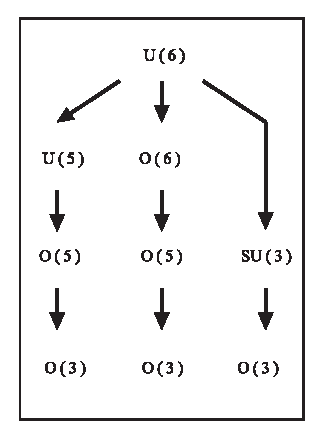
\includegraphics[height=4cm]{figure.eps}
% %
% % If not, use
% %\picplace{5cm}{2cm} % Give the correct figure height and width in cm
% %
% \caption{Please write your figure caption here}
% \label{fig:1}       % Give a unique label
% \end{figure}

% %
% % For tables use
% %
% \begin{table}
% \centering
% \caption{Please write your table caption here}
% \label{tab:1}       % Give a unique label
% %
% % For LaTeX tables use
% %
% \begin{tabular}{lll}
% \hline\noalign{\smallskip}
% first & second & third  \\
% \noalign{\smallskip}\hline\noalign{\smallskip}
% number & number & number \\
% number & number & number \\
% \noalign{\smallskip}\hline
% \end{tabular}
% \end{table}

% % For built-in environments use
% %
% \begin{theorem}
% Theorem text goes here.
% \end{theorem}
% %
% % or
% %
% \begin{lemma}
% Lemma text goes here.
% \end{lemma}
%%%%%%%%%%%%%%%%%%%%%%%% Springer-Verlag %%%%%%%%%%%%%%%%%%%%%%%%%%


%%%%%%%%%%%%%%%%%%%%% chapter.tex %%%%%%%%%%%%%%%%%%%%%%%%%%%%%%%%%
%
% sample chapter
%
% Use this file as a template for your own input.
%
%%%%%%%%%%%%%%%%%%%%%%%% Springer-Verlag %%%%%%%%%%%%%%%%%%%%%%%%%%

\chapter{Processor Allocation and Process Migration}

\section{Problems and Goals}
\paragraph{Scheduling a System}
The discussion involves
\begin{itemize}
    \item pick a processor to run a process
    \item move a process from one processor to another processor
\end{itemize}

\paragraph{Process Migration}
The discussion involves
\begin{itemize}
    \item decide a process that should be migrated.
    \item select a new host for the process
    \item migrate the resource of the process
\end{itemize}

The migration here is talking about process. The threads of one process should be migrated together. We do not discuss that the threads are dispatched on different processors.

\section{Processor Allocation}
You need to be careful when you want to migrate a process. There is a difference between \emph{remote execution} and \emph{processor allocation}. People may not know that their local processes have been migrated to a remote processor and executed remotely.

\subsection{Approaches}

\subsubsection{A Centralized Approach: Up-Down}
There are CPU consumers and suppliers existing in the network. We give credits to the suppliers and take credits from the consumers. The hosts with more credits can have high probability to acquire a CPU.

\subsubsection{Hierarchical Approach}
\paragraph{Goal}
Hierarchical Approach can reduce the communication and information across the network in order to balance the load. 

\paragraph{Method}
There are workers on the leaves, and managers on the inner nodes. If a worker gets too much work or too little work, it will inform the manager above.
\begin{itemize}
    \item The manager will use the information to try a shift between workers of it.
    \item The manager meets the limit of its quotas, then tell the directors who try to balance the load among the managers.
\end{itemize}

\begin{figure}
\centering
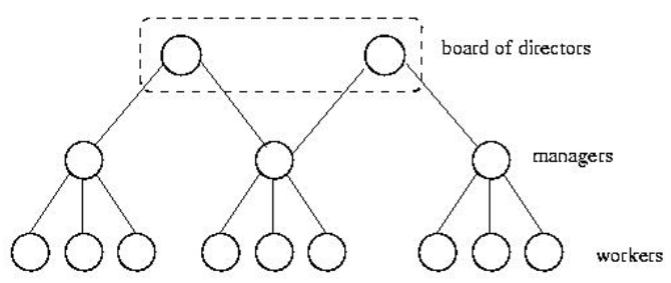
\includegraphics[width=\textwidth]{img/ch02-hier_proc.png}
\caption{Hierarchical Processor Management}
\label{fig:ch02-hier_proc}
\end{figure}

\paragraph{Loads}
We discussed the method for balance loads above that the workers gets too much work or too little work, it will inform managers. But how it communicate the information with managers and workers.

\begin{enumerate}
    \item Yell out. When a worker meets the situation, it yells out to others. If it is idle, it may cause \emph{thundering herds} that everyone wants to use it which makes it busy immediately.
    \item Receiver Initiated. The idle processor asks around. But this approach leads to heavy communications.
    \item Sender Initiated. The busy processor asks around to reduce load.
    \item Hybrid Approach. These try to balance the costs of the above two approaches. They only "yell out" if they are substantially overworked or under worked.
\end{enumerate}

\section{Process Behavior and Scheduling}
In general-purpose systems, recently started jobs are likely to be short lived, whereas long-running jobs are likely to keep running for a very long time.

\section{Process Migration}
Some ideas are here:
\begin{itemize}
    \item Virtual Machine can make the migration easier, but it arises some network problems, such as IP address.
    \item If we want to migrate processes, we need to build a recoverable, portable communication layer (do not hack with TCP). This layer allows suspend, update and resume programs.
    \item There are some systems working for this scheduling: HTCondor, TORQUE.
\end{itemize}

\chapter{Log and Checkpoint}

\section{Problems and Goals}
As for \textbf{recovery}, there are three ways
\begin{itemize}
    \item Replication. It is true that replication can make the system more fault tolerant, but it is expensive and also require a lot of synchronization work.
    \item Checkpoint. If the system make changes (progress), we can make checkpoints to store the system states. But the problem for checkpoint is that the systems need a \textbf{freeze} when backing up. However, we can try to find a consistent recovery line, which will be discussed later.
    \item Log. The classic technique is \textbf{Write Ahead Logging}. Events need to be written in the log first before executed.
\end{itemize}

For cooperation between checkpoint and log, we use logs between checkpoints. Recovery involves checkpointing and logging. Checkpoints store the state of process, logging involves recording the operations that produced the current state.

\section{Sender-based Logging}
Sender based logging is very important in those cases where receivers are thin or unreliable. In other words, we would want to log messages on the sender if the receiver does not have the resources to maintain the logs, or if the receiver is likely to fail. 

\subsubsection{Ensure that the order in both senders and receivers are correct.}

Senders can play back the logging in the same order in which they were dispatched.It is difficult to order the messages from senders in the receiver side.

To ensure this, we follow the protocol:
\begin{itemize}
    \item The sender logs a message and send it.
    \item The receiver gets the message and ACKs it with the time local to the receiver.
    \item The sender adds this timestamp in the ACK into that log entry.
\end{itemize}
Under this protocol, we can resend the message with the order recorded by the senders when dispatching. At the same time, when messages arrive the receivers, they can also order the messages with the receivers' time stamp.

\subsubsection{Ensure the sender get the timestamped ACKs from receivers (make sure logs are complete)}

Require the sender to send a ACK-ACK to the receiver before send a following message. 
\begin{figure}
\centering
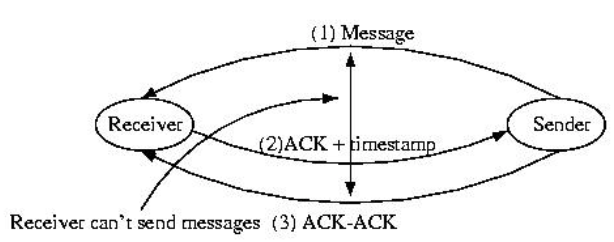
\includegraphics[width=\textwidth]{img/ch03-log_ackack.png}
\caption{ACK-ACK log.}
\label{fig:ch03-log_ackack}
\end{figure}

Before the receiver gets the ACK-ACK for the first message, it cannot send messages to the sender. It make sure that we get the correct order in the receiver side.

\section{Recovery from Failure}
Recovery involves sending lots of history messages. \textbf{Duplicate messages} are the messages sent to other normal systems. \textbf{Orphan messages} are that after a rollback some systems may receive the messages that the recovering system does not remember sending. Rollback to a fail system may causes another system to rollback, which is known as \textbf{cascading rollbacks}. Eventually the systems will reach a state where they can move forward together, which is known as \textbf{recovery line}. After a rollback, a system may duplicate output, or request the input again, which is called \textbf{studdering}.

\subsection{Incarnation Numbers}
\textbf{Incarnation} is the period between checkpoints. Rebooting a system or restarting a cooperating process results in a new incarnation. We can number these incarnations. This number can be used to eliminate duplicate messages.

When a system is reincarnated, it sends a message to the cooperating systems informing them of the new incarnation number. The incarnation number is also send out with all messages. Therefore, the receivers can determine whether or not it is a duplicate message.

\textbf{How the receiver handles the incarnation numbers?}
\begin{itemize}
    \item If the incarnation number of the message is less than the expected number, the message is a duplicate, so it should be discarded.
    \item If the incarnation number is in the message is greater than the expected number, the sender is recovering, so block accepting messages, until it informs us about its new incarnation number. (Maybe because the sender gets the recovery incarnation number first from the sender.)
    \item If they are the same, accept the message.
\end{itemize}

\subsection{Checkpoint: consistency}
The checkpoints of all the servers are unnecessary consistent. Therefore, we need to find a maximum recovery line.

\subsubsection{Interval Dependency Graph (IDG)}
The graph is constructed by creating a node for each interval, and then connecting subsequent intervals on the same processor by constructing an edge from a predecessor to its successor. Then an edge is draw from each interval during which one or more messages were received to the interval or intervals during which the message(s) was or were sent.
\begin{figure}
\centering
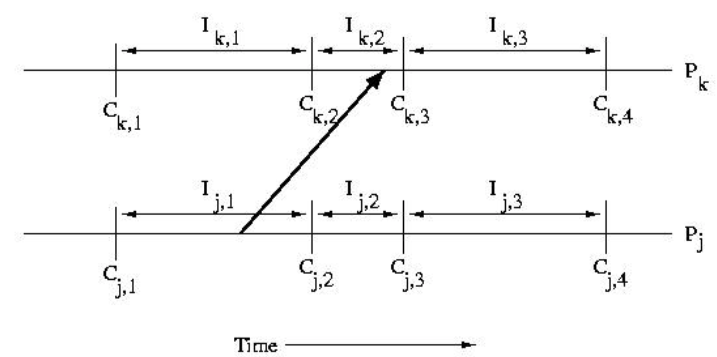
\includegraphics[width=\textwidth]{img/ch03-idg.png}
\caption{IDG}
\label{fig:ch03-idg}
\end{figure}

\textbf{Where to store the graph?} Each processor keeps the nodes and edges that are associated with it.

\textbf{How to find the recovery line?} If there are some lost intervals, the other servers rollback to a interval that is independent of the lost intervals. And this rollback continues until there is a recovery line established.

\subsubsection{Coordniated Checkpoints}
We can decrease the rollbacks happened in the whole system, by coordinating checkpoints. Actually we only discussed how to use IDG, but not how to implicitly build a IDG. Here is the discussion.

There are two methods:
\begin{itemize}
    \item Record message sequence number (the sender information). If the receiver gets a message, it send back a message to tell the senders to check if they checkpointed since the last time they sent the message. If not, the senders need to checkpoint in order to satisfy the dependency.
    \item Synchronized clock. Each processor creates a checkpoint every T units of time.
\end{itemize}

\section{Logging}

\subsection{Kinds of Logging}

\begin{itemize}
    \item Synchronous Logging. Logging before execution. It is expensive and slow.
    \item Asychronous Logging. Occasionally write the logs. Some messages may be logged, while others may not be logged.
\end{itemize}

\subsection{One Approach For Asychronous Logging: GDM}
First, the system maintains a \textbf{Global Dependency Matrix (GDM)}, each processor has a vector recording the interval numbers of processors it knows. 

\begin{figure}
\centering
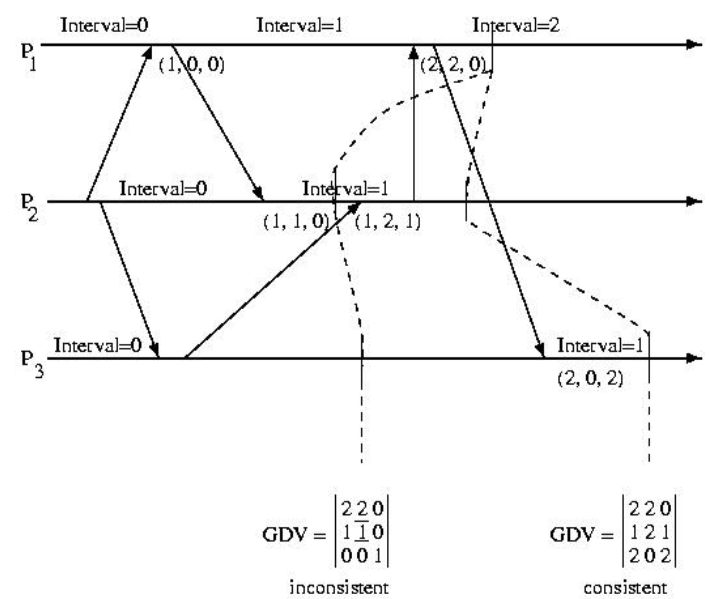
\includegraphics[width=\textwidth]{img/ch03-log_gdv.png}
\caption{GDM}
\label{fig:ch03-log_gdv}
\end{figure}

We can check if the matrix is consistent. The method is similar as before. You can check if the number on the processor's self is the greatest.

The method to find a new recovery line:
\begin{enumerate}
    \item Get the previous recovery line and new updates after the recovery line.
    \item Check for each update, if it can hold a consistent state for the system. If so, update the recovery line and go on checking.
\end{enumerate}

\subsection{Adaptive Logging}
We do not need to log every message. It only needs to log those messages that have originated from processors that have taken checkpoints more recently than it has. Before there are new updates existing on the senders. If the receiver is ahead, it won't worry about it and do not need to checkpoint.


\chapter{MapReduce and Hadoop}

\section{Problems and Goals}
\begin{itemize}
    \item How many maps
    \item How many reduces
    \item Locality, replication
    \item Combining Maps and Reduces: combiner only reduce the size of results from Maps, and the results are written in an intermediate file. 
    \item Worker failure. When a Map worker dies, it needs to be re-executed from scratch. The reason for this is the results are stored on the Worker's local disk and are now inaccessible to Reduces. But, should a Reduce Worker fail, its results remain available in the global file system.
    \item Master failure. The master isn't scaled up. It is just one central Master. Like your desktop. Failures are years apart. And, checkpointing things will waste tons of time. Instead, if a computation times out, the program can just restart the computation a new, perhaps after checking the status of and with the Master.
    \item How many Map-Reduce phases is optimal? You can say it is one. But in reality, it is not possible and also not necessary.
\end{itemize}
% \include{chapter}
%\appendix
%\include{appendix}

% \backmatter%%%%%%%%%%%%%%%%%%%%%%%%%%%%%%%%%%%%%%%%%%%%%%%%%%%%%%%
% 
\chapter*{Solutions}
\addcontentsline{toc}{chapter}{Solutions}
\markboth{Solutions}{Solutions}

\section*{Problems of Chapter~\ref{intro}}

\begin{sol}{prob1}
The solution is revealed here.
\end{sol}


\begin{sol}{prob2}
\textbf{Problem Heading}\\
(a) The solution of first part is revealed here.\\
(b) The solution of second part is revealed here.
\end{sol}


% \include{references}
% \printindex

%%%%%%%%%%%%%%%%%%%%%%%%%%%%%%%%%%%%%%%%%%%%%%%%%%%%%%%%%%%%%%%%%%%%%%

\end{document}





